\documentclass{article}

% Language setting
% Replace `english' with e.g. `spanish' to change the document language
\usepackage[english]{babel}

% Set page size and margins
% Replace `letterpaper' with`a4paper' for UK/EU standard size
\usepackage[letterpaper,top=2cm,bottom=2cm,left=3cm,right=3cm,marginparwidth=1.75cm]{geometry}

% Useful packages
\usepackage{amsmath}
\usepackage{graphicx}
\usepackage{float}
\usepackage[colorlinks=true, allcolors=blue]{hyperref}
%adding bibliography
\usepackage{biblatex}
\addbibresource{bibliography.bib}

\title{Cash-flow maturity and risk premia in CDS markets.}
\author{Antonio Pineda, Nidhi Beeravolu, Kausthub Keshava and Diana Castellanos}

\begin{document}
\maketitle

\section{Introduction}

The project is an academic exercise designed to replicate and analyze the Credit Default Swap (CDS) returns specified by \cite{kelly2017}. The dataset, sourced from the repositories of Markit on Wharthon Research Data Services (WRDS), provides the data foundation upon which our replication model is constructed. Supplementary data used in intermediate calculations are sourced from the Federal Reserve's official website and from the Fred website as well. \\

This work is designed to not only corroborate the work of \cite{kelly2017} but also to substantiate the theoretical implications proposed by \cite{Palhares2013} concerning the maturities of cash-flows and their correlation with the risk premia observed in the market for credit default swaps.\\

The primary drawback encountered in our analysis was the lack of clarity provided by the original paper regarding the portfolio construction methodology for the designated 20 portfolios. The documentation did not clearly articulate the method utilized for amalgamating the spreads, leaving significant ambiguity around several key variables. Notably, the absence of notional amounts presented a challenge for adopting a market-weighted approach to combine spreads effectively. Furthermore, the paper did not address how multiple contracts issued by the same entity were managed, nor did it clarify whether all issuances at a given time were considered. The methodology for managing outlier spreads also remained opaque, contributing to the overall lack of transparency in the portfolio construction process.\\

Despite these challenges, our efforts yielded notable successes. We were able to meticulously extract and accurately replicate the rate term structure as delineated in the paper. Additionally, our analysis achieved a close replication of returns for later years within the provided data set.\\

The organization of the paper is as follows: Section 2 elucidates the CDS returns model, outlining the theoretical framework and mathematical foundations that inform our analysis. In Section 3, we describe the data obtained from Markit, providing summary statistics that shed light on the dataset's properties and the prevailing market trends. Section 4 examines the estimated CDS returns, applying the proposed model to assess the dataset and interpret the findings. The conclusion in Section 5 establishes that this study aligns with the trends identified in Kelly (2017), showing similar patterns in the results. While the post-2008 estimated CDS returns generally match the actual returns, portfolios with higher returns exhibit an escalating discrepancy.


\section{Credit Default Swap Returns Model}

According to  \cite{Palhares2013}, CDS returns are definite as:

\begin{equation}
    CDS_{t}^{ret} = \frac{CDS_{t-1}}{250} + \Delta CDS_{t} \times RD_{t-1}
\end{equation}

The right-hand side of the equation is composed of two parts: the carry component and the capital gain return. \

The carry component reflects the return accrued from the seller’s receipt of insurance premium payments. The second term represents the capital gain return, which is calculated by multiplying the change in the credit default swap (CDS) spread by the lagged risky duration of the contract, denoted as \( RD_{t-1} \). This risky duration adjusts the future CDS spread received by the seller to its present value. When this value is multiplied by the change in spread, it estimates the logarithmic capital gain for the seller who is in a short position.\\

The risky duration for CDS of maturity $M$ years with quarterly premium payments is computed as


\begin{equation}
RD_t = \frac{1}{4} \sum_{j=1}^{4M} e^{-\frac{j\lambda}{4}} \cdot e^{-\frac{j(r_{\frac{j}{4}, t})}{4}},
\end{equation}




where:\


$e^{-\frac{j\lambda}{4}}$ is the quarterly survival probability, \ 

$r^{\frac{j}{4}}_t$ is the risk-free rate for the quarter $\frac{j}{4}$,\

and $e^{-j\frac{j(r^{\frac{j}{4}})}_{4}}$ is the quarterly discount function.  $\lambda$ for all periods is calculated from the 5-year spread as

\[
\lambda = 4 \log \left(1 + \frac{\text{CDS}}{4L}\right),
\]

where $\text{CDS}$ is the spread and $L$ is the loss given default (assumed to be 60\%). The risk-free term structure is constructed using swap rates for maturities 3 and 6 months and US Treasury yields for maturities from 1 year to 10 years.


\section{Automated Data Fetch and Processing}
In this section, We first describe the data sources that we use and give an overview of the data. Then we present the calculation of CDS returns.


We use the Par Spread data corresponding to a five-year tenor sourced from CRSP, spanning the years 2001 to 2024, for our analysis of Credit Default Swap (CDS) spreads. This dataset encompassed all available tickers, which we then categorized into quantiles based on CDS spreads to form our portfolios. The spreads within each portfolio is combined through different methods to form a series of CDS spreads for each of the 20 portfolios. We explored three separate methods of combining the individual tickers within each quantile as the paper does not provide a clear methodological process for doing so. The three techniques we implemented were combining via: (1) Mean of the CDS spreads within each quantile, (2) Median of the CDS spreads within each quantile, (3) Weighted average of the CDS spreads within each quantile where the weights are as per the spreads. Additionally, we applied a smoothing technique specifically to the portfolio corresponding to the 20th quantile due to large variation observed in the series. Below we present the box plot of the CDS returns across the 20 portfolios. It is evident that the spreads are higher for the higher quantiles, which is consistent with the expected behavior based on the construction methodology we performed.

%insert graphs
%![Image Description](../assets/cds_box_plot.png) 

\begin{figure}[H]
    \centering
    \includegraphics[width=0.75\textwidth]{../assets/cds_box_plot.png}
    \caption{\label{fig:cds_rates_box}Box plot of CDS spread across 20 portfolios.}
    
    \end{figure}

    For the short term rates of 3-6 months we fetched data from the Fred website and for rates of maturities between 1-10 years, we used the FED website, and subsequently filtered by the date indices of the CDS dataset. We used the risk free rates for maturities 3 and 6 months and US Treasury yields for maturities from 1 year to 10 years. 
    We extrapolated these rates to quarterly frequency with a cubic spline function. This is a popular technique for datafitting, as this is a smooth approximation to the real value. More details on cubic spline extrapolation has been provided in the project guide. 
    Figure \ref{fig:interest_raw} shows the box plot of interest rates from 3 to 120 months (10 years) and Figure \ref{fig:interest_spline} shows the extrapolated interest rates. We discretize the interest rates to quarterly frequency to match the CDS returns data.
\begin{figure}[H]
    \centering
    \includegraphics[width=0.75\textwidth]{../assets/rates_boxplot.png}
    \caption{\label{fig:interest_raw}Box plot of interest rates from 3 to 120 monts (10 years).}
    \end{figure}

\begin{figure}[H]
    \centering
    \includegraphics[width=0.75\textwidth]{../assets/extrapolated_interest_Rates.png}
    \caption{\label{fig:interest_spline}Extrapolated interest rates.}
    \end{figure}    


\section{Credit default swap returns estimation}
Following equation (1), (2) and the fact that, according to \cite{kelly2017}, the CDS returns definition is assuming a short CDS strategy. The calculation framework has two key pillars:

1) Calibrate the risky durations for each portfolio of CDS products. This concept of risky duration is to capture the credit risk present in an interest rate sensitive product. The usual way we understand duration for a fixed income security is that it is the interst rate sensitivity. He Kelly uses Palhares concept of risky duration which brings in the credit risk component into duration by utilizing a loss given default parameter (assumed to be 0.6) and the CDS spreads themselves. 

2) Combine the risky durations with change in the CDS spreads to calculate the CDS returns. 

The returns calculated through each method (mean, median and weighted average) for each of the 20 portfolios are presented below.  
Figure \ref{fig:returns_box_plot_median} shows the box plot of CDS returns across the 20 portfolios using the median method. Figure \ref{fig:returns_box_plot_mean} shows the box plot of CDS returns across the 20 portfolios using the mean method. Figure \ref{fig:returns_box_plot_weighted} shows the box plot of CDS returns across the 20 portfolios using the weighted average method. It is evident that the returns are higher for the higher quantiles, which is consistent with the expected behavior based on the construction methodology we performed. Moreover, the returns are most volatile for the weighted average method as compared to the mean and median methods.
Below we present the CDS returns estimated for each portfolio using the three methods alongwith the returns calculated in the paper.
\begin{figure}[H]
    \centering
    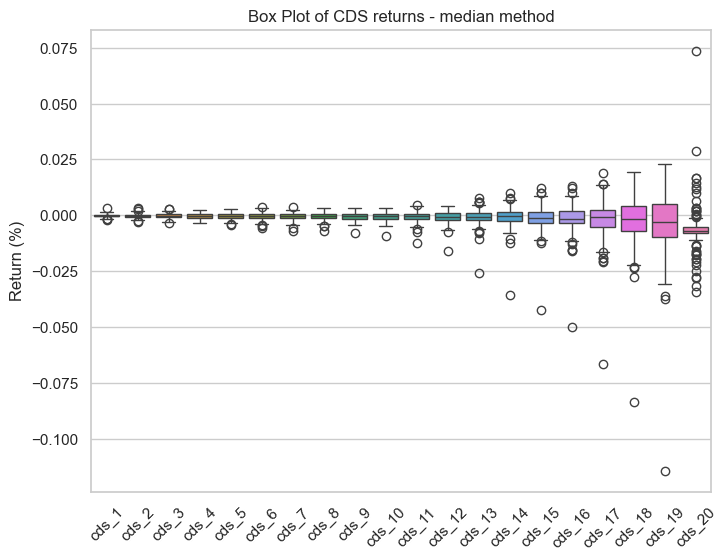
\includegraphics[width=0.75\textwidth]{../assets/cds_returns_boxplot_median.png}
    \caption{\label{fig:returns_box_plot_median}CDS returns estimation with median method}
    \end{figure}

\begin{figure}[H]
    \centering
    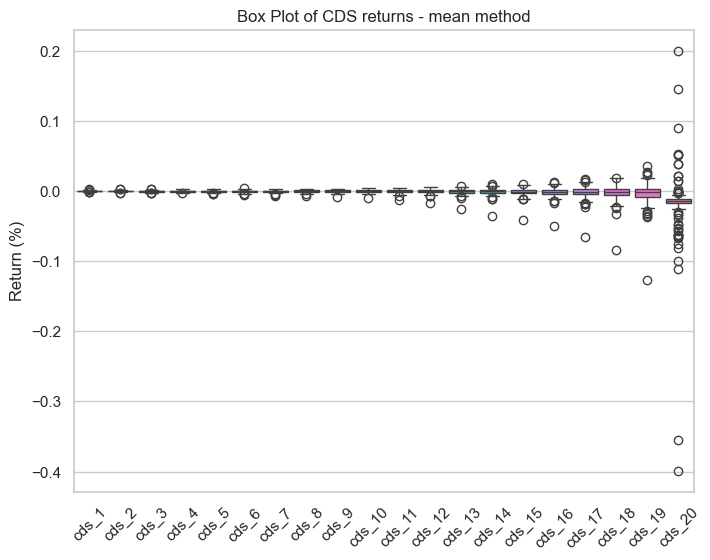
\includegraphics[width=0.75\textwidth]{../assets/cds_returns_boxplot_allportfolios.png}
    \caption{\label{fig:returns_box_plot_mean}CDS returns estimation with mean method}
    \end{figure}   

\begin{figure}[H]
    \centering
    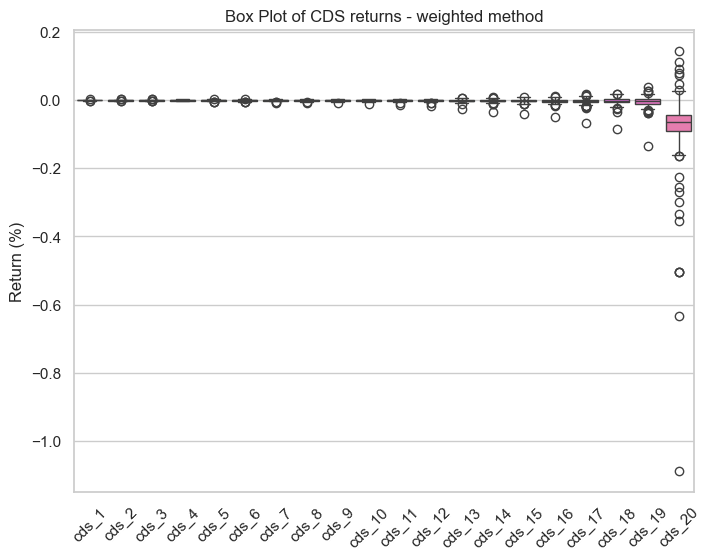
\includegraphics[width=0.75\textwidth]{../assets/cds_returns_boxplots_weighted.png}
    \caption{\label{fig:returns_box_plot_weighted}CDS returns estimation with weighted method}
    \end{figure}       

The project aim was to replicate the CDS returns calculated in \cite{kelly2017}. A key challenge we faced was the lack of clarity in the paper on how the CDS returns were calculated. We had to make assumptions and use our judgement to fill in the gaps. We also had to make assumptions on how to combine the CDS spreads within each quantile to form the CDS returns. We used three methods to combine the CDS spreads within each quantile and calculated the CDS returns. We then evaluate the differences between the actual and computed returns by employing various methodologies. 

\begin{figure}[H]
    \centering
    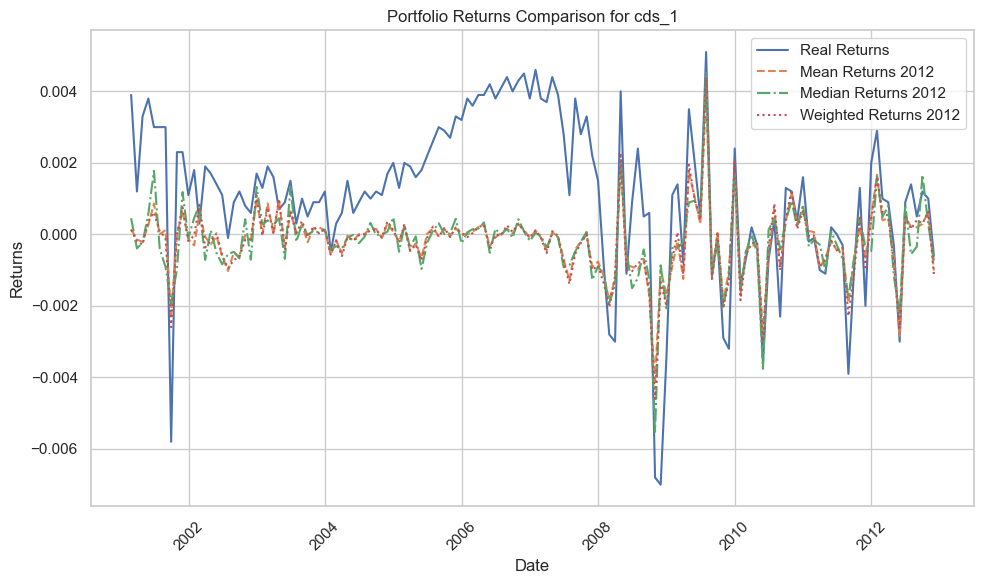
\includegraphics[width=0.75\textwidth]{../assets/returns_cds1_insample.png}
    \caption{\label{fig:cds_rets_p1}Portfolio 1 CDS returns}
    \end{figure}

\begin{figure}[H]
    \centering
    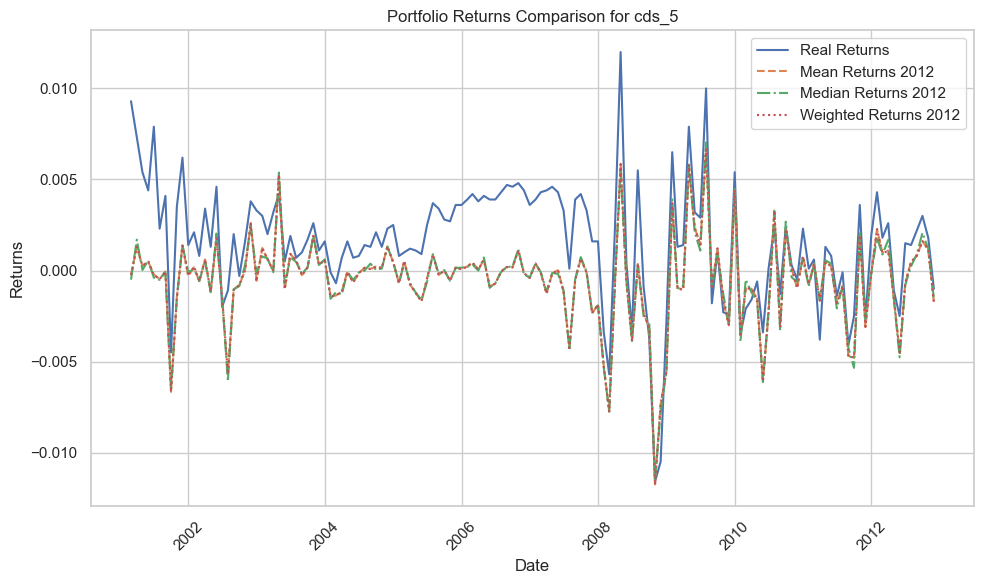
\includegraphics[width=0.75\textwidth]{../assets/returns_cds5_insample.png}
    \caption{\label{fig:cds_rets_p5}Portfolio 5 CDS returns}
    \end{figure}    

\begin{figure}[H]
    \centering
    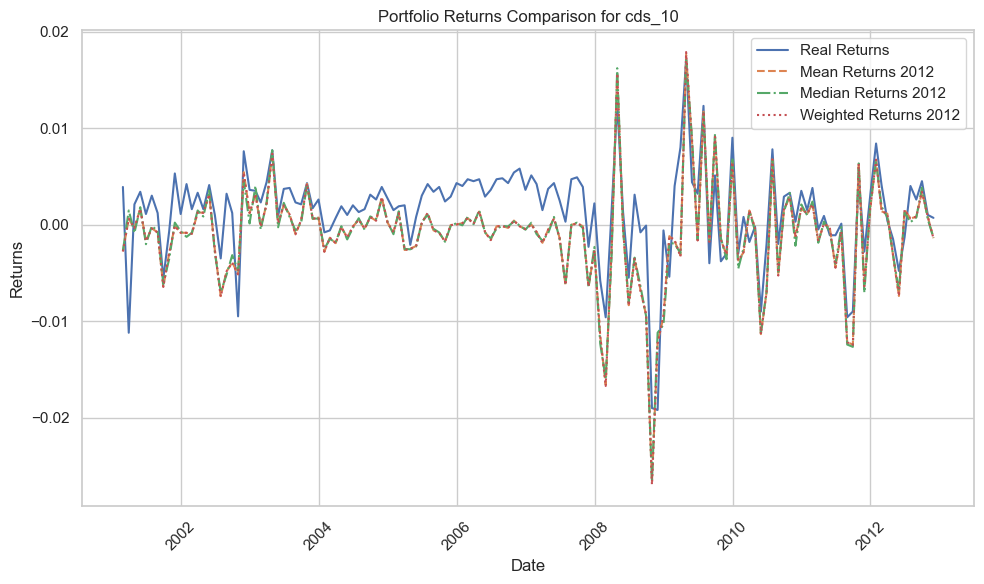
\includegraphics[width=0.75\textwidth]{../assets/returns_cds10_insample.png}
    \caption{\label{fig:cds_rets_p10}Portfolio 10 CDS returns}
    \end{figure}

\begin{figure}[H]
    \centering
    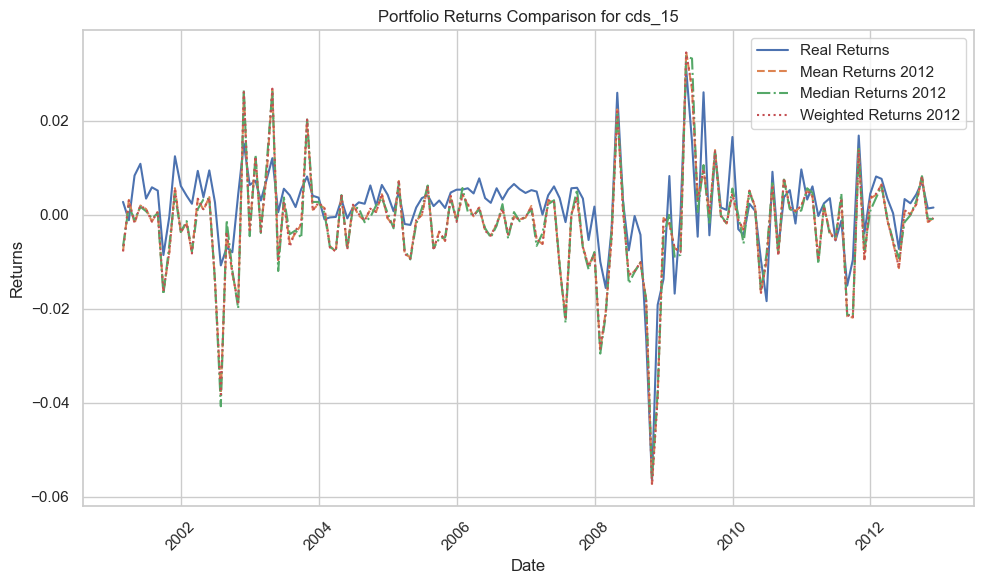
\includegraphics[width=0.75\textwidth]{../assets/returns_cds15_insample.png}
    \caption{\label{fig:cds_rets_p15}Portfolio 15 CDS returns}
    \end{figure}          

\begin{figure}[H]
    \centering
    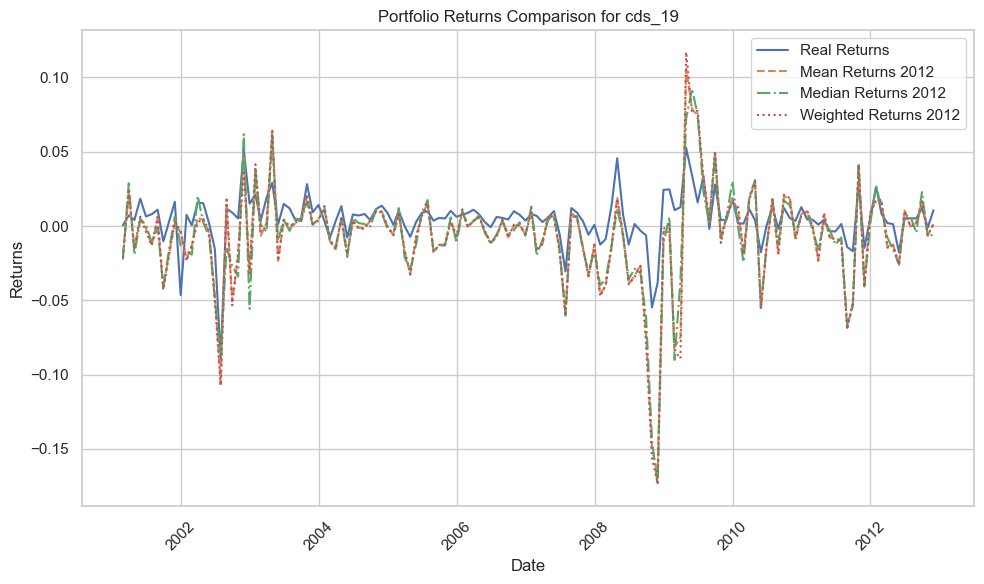
\includegraphics[width=0.75\textwidth]{../assets/returns_cds19_insample.png}
    \caption{\label{fig:cds_rets_p19}Portfolio 19 CDS returns}
    \end{figure}   

\begin{figure}[H]
    \centering
    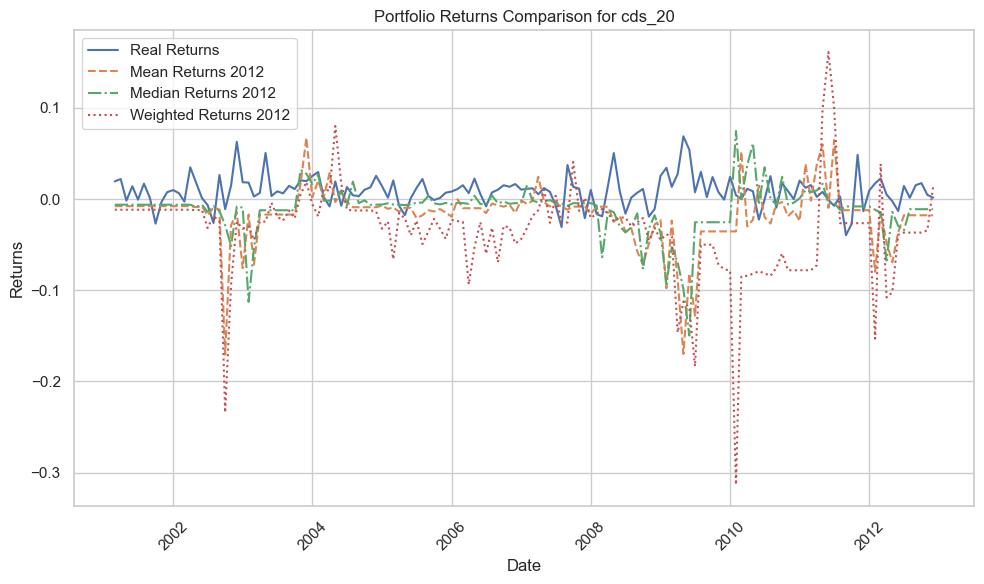
\includegraphics[width=0.75\textwidth]{../assets/returns_cds20_insample.png}
    \caption{\label{fig:cds_rets_p20}Portfolio 20 CDS returns}
    \end{figure}   


Starting in 2008, the computed returns closely align with the real returns, with the exception of cds\_20.\\ 

This particular case stands out as an outlier due to its significantly higher spreads, known for their unpredictability. The paper does not provide clarity on how this anomaly was addressed, leading to the observed discrepancies in results.\\

We evaluate the discrepancy between the actual and computed returns by employing various methodologies. The accompanying tables illustrate that, for the entire sample period, the average error remains under 1\% for the majority of the portfolios. Notably, the largest errors are observed in cds\_19 and cds\_20.

\begin{figure}[H]
    \centering
    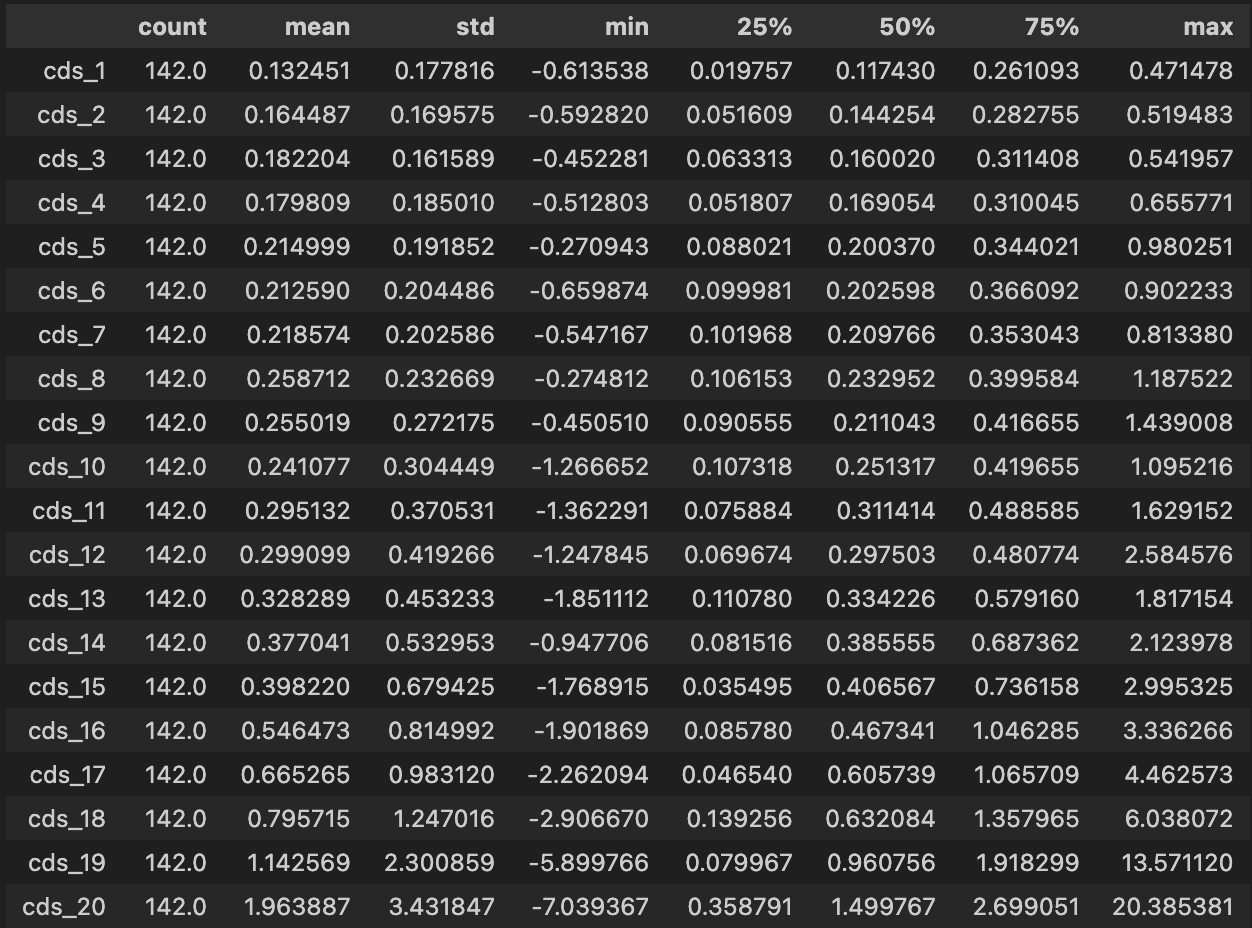
\includegraphics[width=0.75\textwidth]{../assets/Return difference_median method.png}
    \caption{\label{fig:myplot}Estimation error with median method.}
    \end{figure}          

\begin{figure}[H]
    \centering
    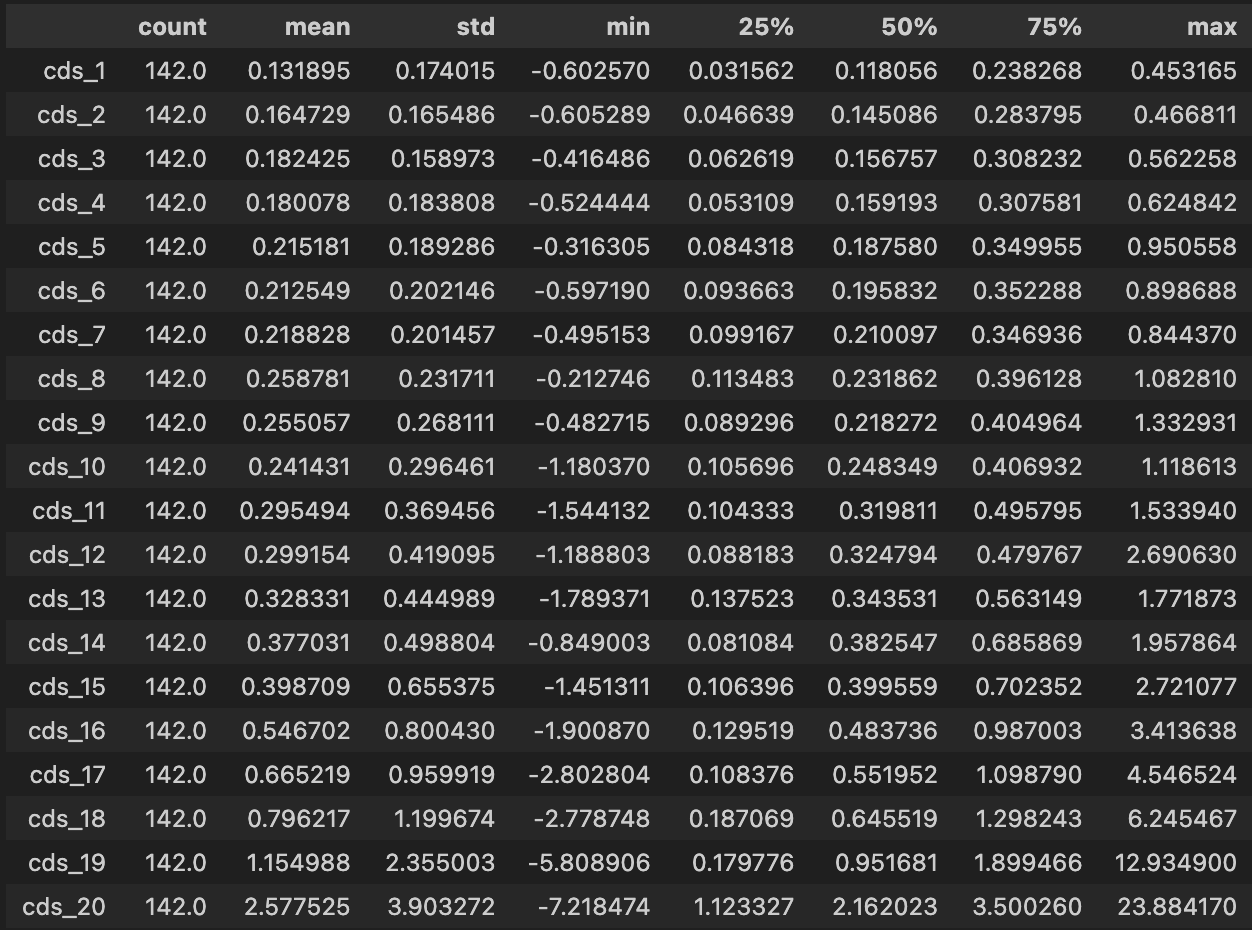
\includegraphics[width=0.75\textwidth]{../assets/Return difference_mean method.png}
    \caption{\label{fig:myplot}Estimation error with mean method.}
    \end{figure}   

\begin{figure}[H]
    \centering
    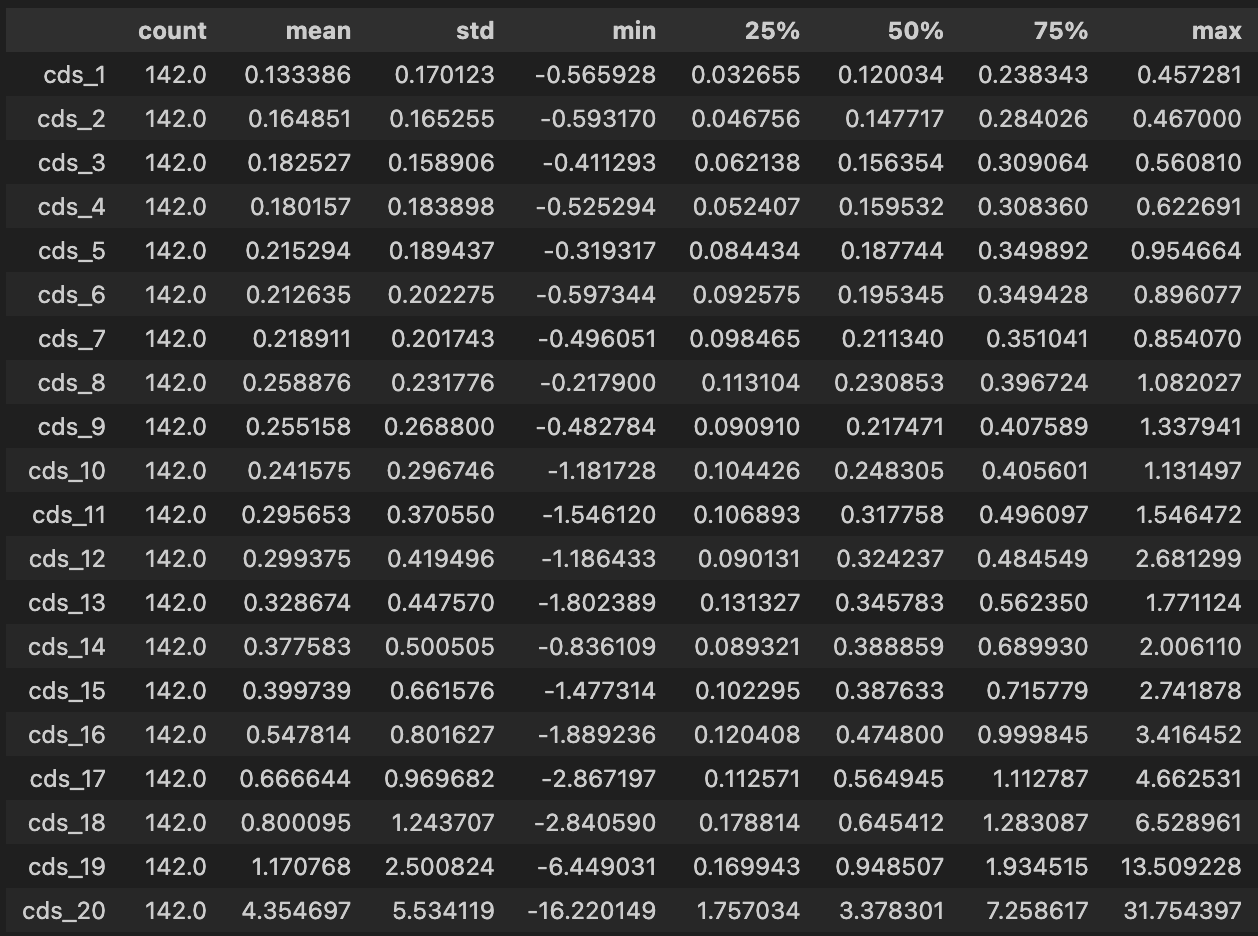
\includegraphics[width=0.75\textwidth]{../assets/Return difference_weighted method.png}
    \caption{\label{fig:myplot}Estimation error with weighted method.}
    \end{figure} 



\subsection*{CDS returns from 2012 onwards}

The CDS returns estimations out sample for each method (mean, median and weighted average) are:

\begin{figure}[H]
    \centering
    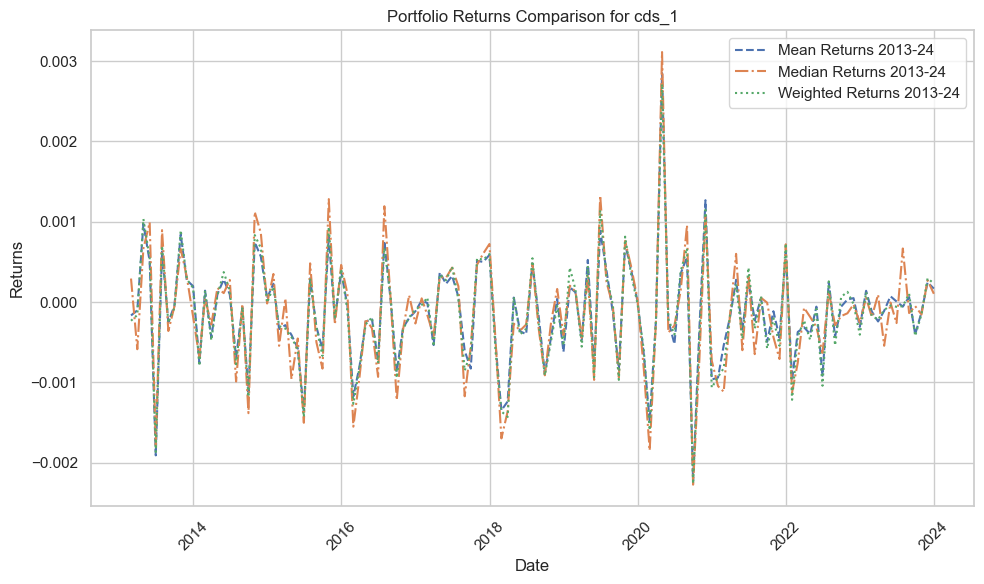
\includegraphics[width=0.75\textwidth]{../assets/returns_cds1_2013_2024.png}
    \caption{\label{fig:myplot}Portfolio 1 CDS returns estimated outsample.}
    \end{figure}

\begin{figure}[H]
    \centering
    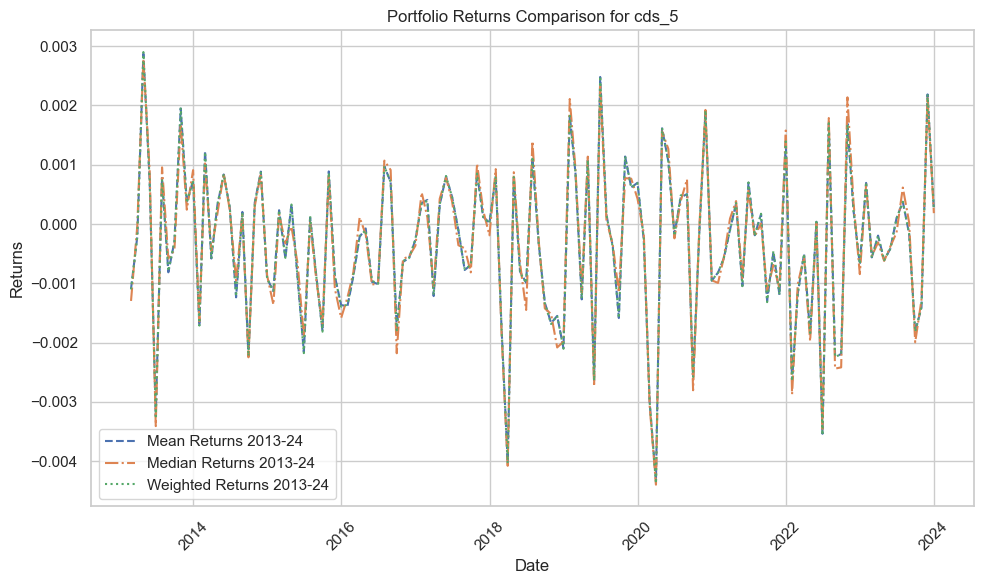
\includegraphics[width=0.75\textwidth]{../assets/returns_cds5_2013_2024.png}
    \caption{\label{fig:myplot}Portfolio 5 CDS returns estimated outsample.}
    \end{figure}    

\begin{figure}[H]
    \centering
    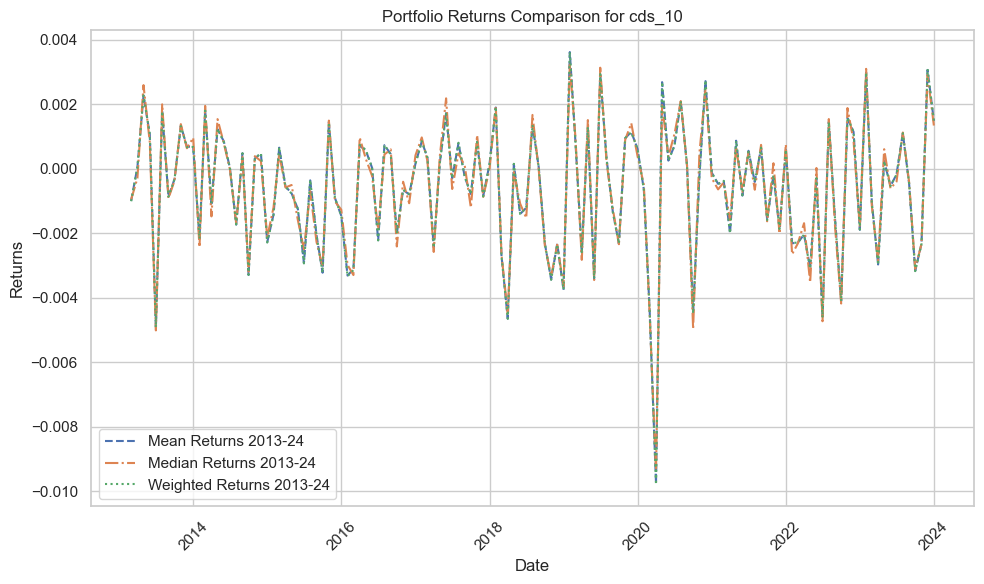
\includegraphics[width=0.75\textwidth]{../assets/returns_cds10_2013_2024.png}
    \caption{\label{fig:myplot}Portfolio 10 CDS returns estimated outsample.}
    \end{figure}

\begin{figure}[H]
    \centering
    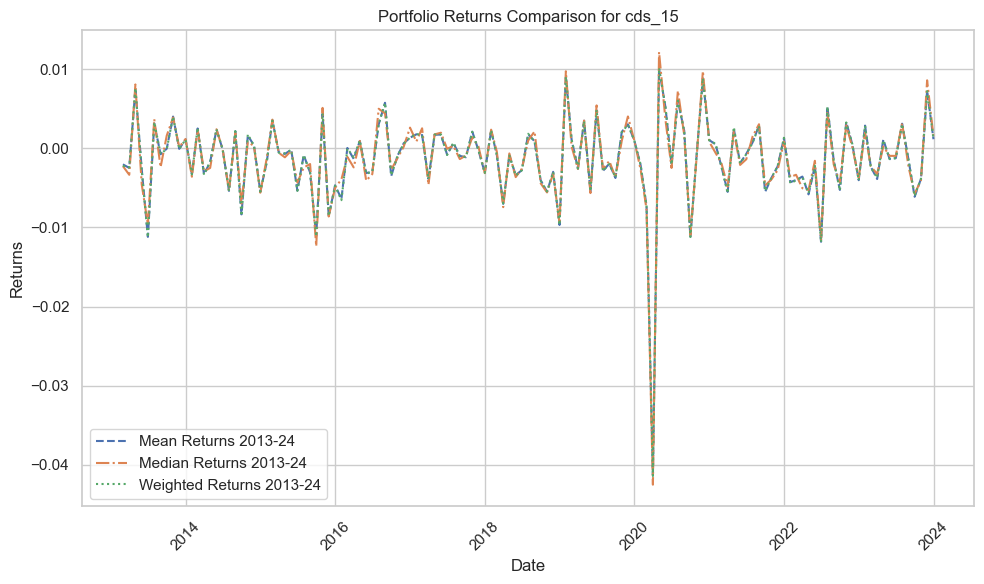
\includegraphics[width=0.75\textwidth]{../assets/returns_cds15_2013_2024.png}
    \caption{\label{fig:myplot}Portfolio 15 CDS returns estimated outsample.}
    \end{figure}          

\begin{figure}[H]
    \centering
    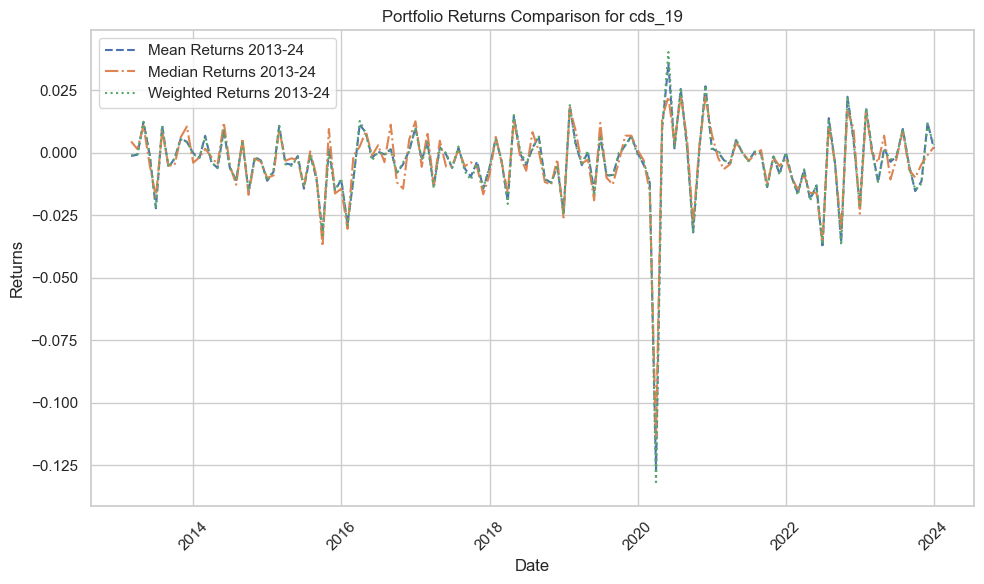
\includegraphics[width=0.75\textwidth]{../assets/returns_cds19_2013_2024.png}
    \caption{\label{fig:myplot}Portfolio 19 CDS returns estimated outsample.}
    \end{figure}   

\begin{figure}[H]
    \centering
    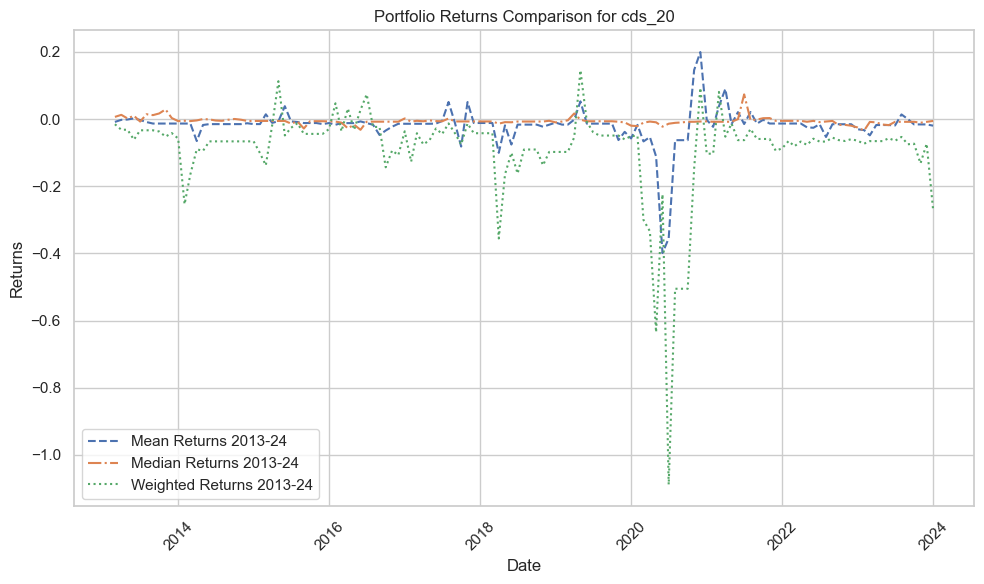
\includegraphics[width=0.75\textwidth]{../assets/returns_cds20_2013_2024.png}
    \caption{\label{fig:myplot}Portfolio 20 CDS returns estimated outsample.}
    \end{figure}   
    

\section{Conclusion.}

In conclusion, our research echoes the observations of Kelly (2017), demonstrating analogous patterns in the results. After 2008, our model's estimates of CDS returns align closely with the actual figures, with the notable exception of portfolios in the higher quantiles, such as cds\_{19} and cds\_{20}. The lack of a detailed methodological explanation in the original study for addressing these outliers contributes to the discrepancies we observe in the outcomes.\\

Among the methodologies evaluated for calculating CDS returns, the approach employing the median-based calculation demonstrated superior accuracy across the entire sample period, particularly for portfolios characterized by wider CDS spreads. This finding suggests that the median method provides a more robust mechanism for capturing the intrinsic value movements within CDS portfolios, especially in scenarios involving greater credit risk. \\

Given these insights, future research might benefit from further refinement in portfolio construction techniques and the calculation of risky duration. Specifically, adjusting the lambda parameter to reflect a more precisely estimated default intensity could enhance the accuracy of risky duration computations. Such improvements hold the potential to refine our understanding of CDS returns, contributing to more informed investment decisions and risk management practices in the CDS market.\\

\bibliographystyle{alpha}
\bibliography{bibliography}

\end{document}